\subsection{Oscillatore a rilassamento}
In questa parte dell'esperienza studieremo il funzionamento di un oscillatore a rilassamento. Tale circuito sfrutta l'instabilità della retroazione positiva per generare un segnale oscillante con una frequenza determinata dai componenti stessi del circuito. In Fig.(\ref{suca}) è riportato lo schema circuitale. 

\begin{wrapfigure}[28]{H}{0.7\textwidth}
	\begin{center}
		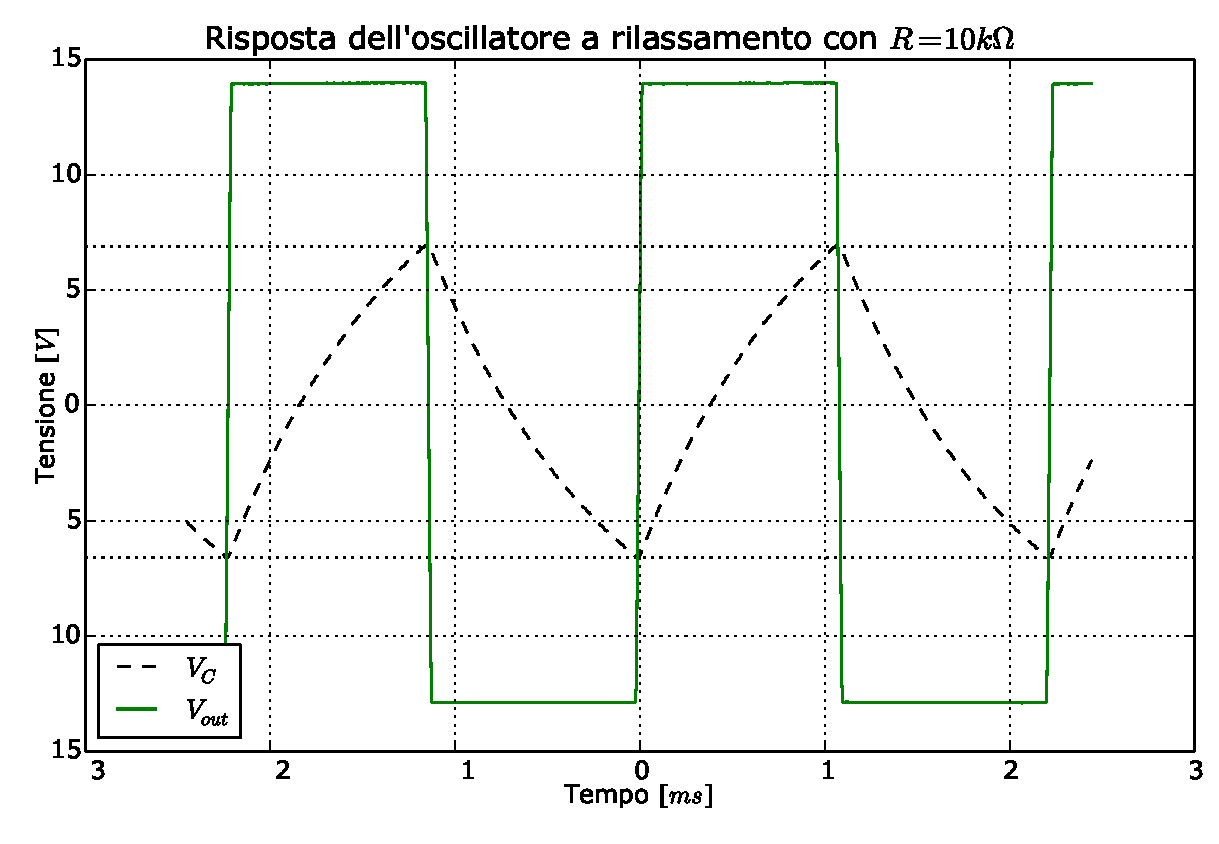
\includegraphics[width=0.7\textwidth]{../E04/latex/osc10k.pdf}
	\end{center}
	\caption{Cricuito oscillatore a rilassamento con C=$(85\pm0.5) \si{\nano\farad}$, $R=(9.99\pm0.01)\si{\kilo\ohm}$, $R_2=(9.96\pm0.01)\si{\kilo\ohm}$ e $R_2=(9.98\pm0.01)\si{\kilo\ohm}$.}
	\label{gr4:osc10k}
\end{wrapfigure}



L'elemento circuitale fondamentale per il funzionamento dell'oscillatore a rilassamento è il condensatore C. Per comodità a $t=0$ assumiamolo scarico e $V_{out}=+V_{sat}$. Ovviamente, per effetto della retroazione negativa, la tensione all'ingresso invertente tenderà ad aumentare ($V_{inv}$ è determinata da quanta carica è accumulata sul condensatore). Non appena $|V_{inv}|>|V_{ninv}|$, avremo uno switch della tensione in uscita, ovvero $+V_{sat} \rightarrow -V_{sat}$. Il condensatore inizierà dunque a scaricarsi. Successivamente avremo un altro swich della tensione in uscita e il ciclo si ripeterà. Il periodo di tale oscillazione può essere calcolato analiticamente risolvendo il circuito. Il valore che si ottiene è $T=2RCln(1+\frac{2R_1}{R_2})$.  





Nel grafico sono riportati i risultati ottenuti per valori di $R=(9.99\pm0.01)\si{\kilo\ohm}$. Come vediamo, carica e scarica del condensatore tendono a $\pm V_{sat}$.




Nella seguente tabella riportiamo i valori teorici e sperimentali di periodo dell'oscillatore a rilassamento.

\begin{tabular}{|l|l|l|}
\hline
$R [\si{\kilo\ohm}]$	&  $T_{exp} [\si{\milli\second}]$          & $T_{teo} [\si{\milli\second}]$       \\
\hline
$9.99\pm0.01 $ & $2.22\pm0.01$ & $2.19 \pm 0.03$\\
\hline
$99.93\pm0.01 $ & $22.2\pm0.1$ & $21.9 \pm 0.3$\\
\hline
\end{tabular} 
